
%%%%%%%%%%%%%%%%%%%%%%
%%%%%%%%%%%%%%%%%%%%%%
%\subsection{Multi-functional proteins}
%%%%%%%%%%%%%%%%%%%%%%
%%%%%%%%%%%%%%%%%%%%%%
%
%It is well-known that some proteins have the ability to carry out more than one function, or ``moonlight" \citep{Jeffery1999,Jeffery2009}. Such abilities can be facilitated by either having multiple functional domains, a single domain which binds multiple partners, or by different behavior upon post-translational modifications or change in physiological conditions \citep{Jeffery2004,Jeffery2009}. Here we systematically analyze multi-functionality with respect to Molecular Function (MFO) and Biological Process Ontologies (BPO) in GO. As an approximation of distinct functions we only consider the number of experimentally determined leaf GO terms associated with each protein. A GO term $g$ was included in the count if no other term associated with the protein had $g$ as its more general term in the ontology. For example, if a protein is associated with the term ``protein binding", the term ``binding" is not counted as distinct function because it is a generalization of ``protein binding"; however, the term ``nucleic acid binding" would be counted because neither of the two terms is a generalization of the other.
%
%\Cref{fig:fanngo1} shows the distribution of the number of leaf terms associated with each functionally annotated sequence for both ontologies. In total, $26,707$ sequences were included in the MFO analysis and $29,118$ sequences were included in the BPO analysis (see \Cref{sec:fanngodata}). Only experimental evidence, traceable author's statement, or curator's inference were considered (exclusion of traceable author's statement and curator's inference resulted in very similar distributions; data not shown). The plots show greater diversity in a protein's participation in a biological process than its ability to carry out distinct molecular functions. About $66\%$ of the proteins experimentally annotated by MFO terms have only $1$ leaf term, with no protein having more than $14$. On the other hand, only $44\%$ of proteins have only $1$ BPO leaf term, with $6$ proteins having $50$ terms or more. This is consistent with the expectation that biological processes are governed more by the context in which a protein is utilized, and less by the physicochemical abilities of the protein. Interestingly, both the molecular function and biological process ontologies show a scale free-like decrease in the probability that a protein is associated with an increasing number of functional terms. In the context of protein function prediction, these distributions suggest there is a level of sophistication that should be required from a computational method with respect to its outputs.
%
%%%%%%%%%%%%%%%%%%%%%%
%%%%%%%%%%%%%%%%%%%%%%
%\begin{figure*}[h!]
%\begin{centering}
%
\includegraphics[width=\linewidth]{Figures/fanngo/Figure_1}
%\par\end{centering}
%\caption[The distribution of leaf terms counts per ontology]{The distribution of the number of leaf terms in (A) Molecular Function and (B) Biological Process ontologies. The x-axis represents the number of leaf terms associated with a protein; the y-axis represents the fraction of proteins in the data set with the given number of leaf terms. Both axes are in log10 scale. The inset in each panel provides a pie chart that corresponds to each plot.}
%\label{fig:fanngo1}
%\end{figure*}
%%%%%%%%%%%%%%%%%%%%%%
%%%%%%%%%%%%%%%%%%%%%%
%
%We also analyzed the relationship between the number of molecular functions and biological processes a protein is associated with. It seems intuitive to postulate that proteins with the ability to carry out multiple molecular functions should be more easily utilized in multiple different contexts, giving rise to an association with more biological processes. Out of $19,240$ proteins in the intersection of data sets for molecular function and biological process, we found a Pearson correlation coefficient of $0.261$ between the numbers of associated leaf terms in the two ontologies. While this correlation may seem weak, we determined that this value is statistically significant by using a permutation test where the numbers of MFO and BPO terms were permuted in the data set of proteins. We carried out $100,000$ such permutations and did not find any cases in which the correlation coefficient was $0.261$ or greater (the mean correlation coefficient for permuted data was $6.1\times10^{-6}$ and standard deviation was $7.2\times 10^{-3}$). 
%
%While, in general, a protein performing multiple molecular functions is associated with multiple biological processes, we conducted further analysis of proteins associated with a single term from one ontology and multiple terms from the other. For example, among the proteins that have only one MFO leaf term, but multiple BPO terms, we found that receptor binding terms such as ``chemokine receptor binding" and ``cytokine receptor binding" are the most enriched ($P < 1.0\times10^{-7}$; Binomial test). On the other hand, there are also cases in which proteins that are associated with only one leaf term in BPO are related to multiple MFO terms. Such BPO terms are almost all related to metabolic processes, e.g. ``cellular metabolic process", ``primary metabolic process", etc. ($P < 1.0\times10^{-7}$; Binomial test). When analyzing this class of proteins we also found that some terms did not occur as often as expected.  When looking at the class of proteins with one MFO term and multiple BPO terms we found that ``catalytic activity" was depleted. While sequences are annotated with this term $28\%$ of the time in the whole data set ($29\%$ in the set of all proteins with single MFO leaf term), it only occurs $17\%$ of the time when we only consider sequences with exactly one MFO term but $3$ or more BPO terms associated with them. Similarly, proteins having $1$ BPO leaf term, but few MFO terms are usually involved in reproduction. We note that this data needs to be interpreted with caution, because MFO and BPO terms are incomplete for most proteins and also because there may exist biases in ways current functions are acquired.
%
%Finally, we looked at the relationship between the number of Pfam domains \citep{Finn2008} found in a protein and the number of BPO and MFO terms it was associated with. We found that the Pearson correlation between the number of MFO leaf terms and Pfam domains (detected using a threshold of $0.001$) was much larger than that of BPO leaf terms and Pfam domains ($0.126$ and $0.090$ respectively). While, again, these correlation values might seem small, we found both were significant using the permutation test.
%
%%%%%%%%%%%%%%%%%%%%%%
%%%%%%%%%%%%%%%%%%%%%%
%\subsection{Transfer of function by sequence similarity}
%%%%%%%%%%%%%%%%%%%%%%
%%%%%%%%%%%%%%%%%%%%%%
%
%We evaluated the performance of simple function transfer between similar sequences. The following steps were taken: for each range of pairwise global sequence identities, a target protein received all functional terms from each experimentally annotated protein within the given sequence identity range (regardless of the species). For each target sequence with more than one match in the given identity range the precision and recall (see \Cref{sec:fanngomodels}) were calculated as averages over all pairs. Then, the precision and recall for the entire data set are reported (\Cref{fig:fanngo2}) as averages of the averaged precisions and recalls calculated for each sequence covered (a leave-one-out estimation). We also report the coverage for each range of sequence identity as the fraction of proteins with at least one other annotated sequence whose pairwise sequence identity falls within the defined range. Finally, for all covered sequences we report the percentage of perfect annotations, i.e. the percentage of all pairwise annotations in a given bin where both precision and recall were 1.
%
%%%%%%%%%%%%%%%%%%%%%%
%%%%%%%%%%%%%%%%%%%%%%
%\begin{figure*}[h!]
%\begin{centering}
%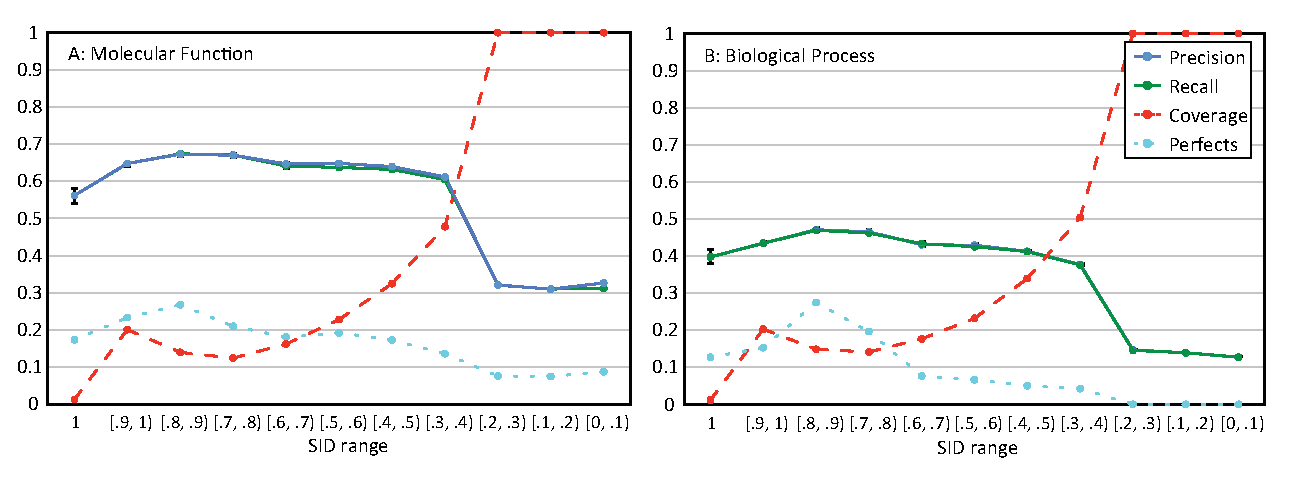
\includegraphics[width=\linewidth]{Figures/fanngo/Figure_2}
%\par\end{centering}
%\caption[Accuracy of function transfer using global sequence identity]{Accuracy of function transfer using global pairwise sequence identities (A: Molecular Function; B: Biological Process). For each sequence identity range (x-axis), shown are the average precision (blue solid line) and recall (green solid line) of function transfer by pairwise similarity. The teal dotted line represents the percentage of pairs with perfect annotations (e.g. both precision and recall equal to 1). The red dashed curve represents the percent of proteins that have pairwise matches (annotated with GO terms; experimental evidence code) in a given range. The error bars represent 95\% confidence intervals.}
%\label{fig:fanngo2}
%\end{figure*}
%%%%%%%%%%%%%%%%%%%%%%
%%%%%%%%%%%%%%%%%%%%%%
%
%The results shown in \Cref{fig:fanngo2} suggest that using global sequence identity for the transfer of functional annotations is only moderately accurate (pairwise local alignments performed similarly; data not shown). Surprisingly, even for $100\%$ identity transfer of function does not achieve either precision or recall of $1$ (only $17\%$ of identical sequence pairs had perfect transfer of MFO and $12\%$ of BPO terms). This relatively low rate of perfect annotations among perfect matches, and similarly in the remaining identity bins, in our data set is caused by three factors: (i) sparsity of database annotations, where proteins are incompletely annotated with respect to functionality and also specificity of annotation; (ii) database errors, caused by incorrect interpretation of experiments or by curation errors, \citep{Brenner1999,Schnoes2009} and (iii) organismal context, where the difference between two organisms influences a particular functional role of individual proteins, even at $100\%$ sequence identity.
%
%In general, transferring MFO annotations is more accurate than transferring BPO annotations, which has previously also been observed by Rogers and Ben-Hur in a different prediction scenario \citep{Rogers2009}. This is probably a result of the fact that MFO terms are less dependent upon cellular, tissue, or organismal context, but also that the topological properties, including the average branching factor, the number of terms, and the average depth of a leaf node, between the two ontologies differ (data not shown). For both ontologies the precision of transferring predictions rapidly decreases once the $20-30\%$ identity is reached. This range of sequence identity has been termed the ``twilight zone" for the inference of protein structure from sequence \citep{Rost1999}. In the context of function transfer such a twilight zone cannot be clearly defined (or rather should be extended to the entire range $30-100\%$), with the range below $30\%$ being one where function transfer breaks down completely (``midnight zone"). We also evaluated an alternative approach where functional terms from all matches in a given identity range were transferred to the target protein and found a very similar level of precision but an increased recall (\Cref{fig:fanngoS1}).
%
%%%%%%%%%%%%%%%%%%%%%%
%%%%%%%%%%%%%%%%%%%%%%
%\begin{figure*}[h!]
%\begin{centering}
%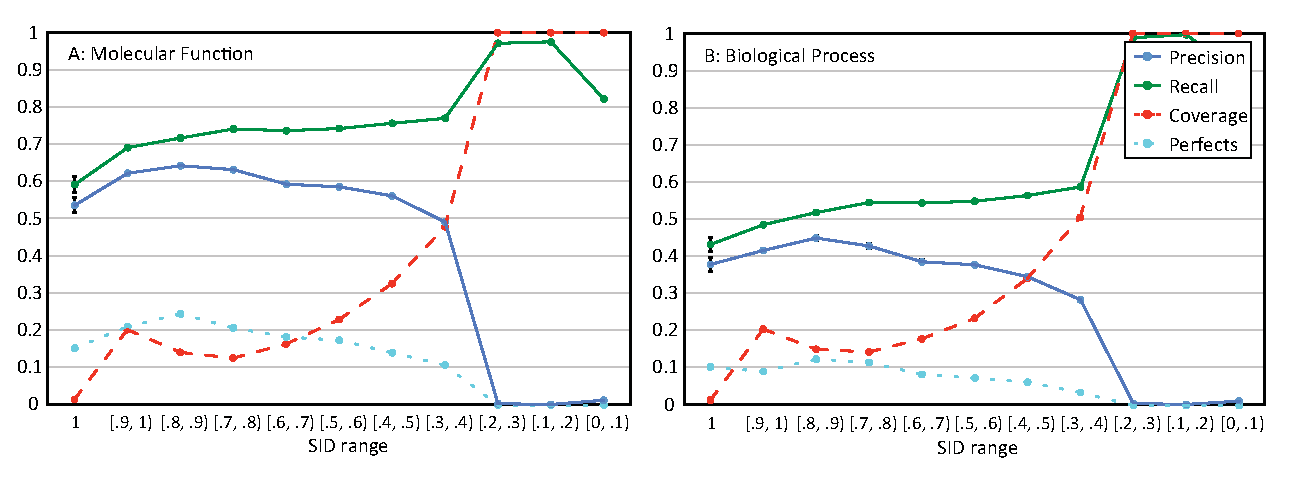
\includegraphics[width=\linewidth]{Figures/fanngo/Supplementary_Figure_1}
%\par\end{centering}
%\caption[The precision and recall of function transfer using global pairwise sequence identities]{The precision and recall of function transfer using global pairwise sequence identities (A: Molecular Function; B: Biological Process). For each sequence identity range (x-axis), shown the average precision (blue solid line) and recall (green solid line) of function transfer were calculated by annotating a target sequence with the annotations of all hits within a particular SID range. The precision and recall curves in this figure differ from those in Figure 2 in that precision and recall for an individual data-point here do not represent an average for each hit, but instead the agglomeration of all terms from hits for a particular range of SID.  The teal dotted line represents the percentage of pairs with perfect annotations (e.g. both precision and recall equal to 1). The red dashed curve represents the percent of proteins that have pairwise matches (annotated with GO terms; experimental evidence code) in a given range. The error bars represent 95\% confidence intervals.}
%\label{fig:fanngoS1}
%\end{figure*}
%%%%%%%%%%%%%%%%%%%%%%
%%%%%%%%%%%%%%%%%%%%%%
%
%The quality of function transfer is highly dependent on the particular class of protein. We show this by splitting the MFO/BPO data sets into enzymes (proteins annotated with term ``catalytic activity"), and non-enzymes. As seen in \Cref{fig:fanngo3}, the ability to transfer molecular functions to these two classes of proteins was noticeably different and most likely points to a higher quality of functional annotations for enzymes.
%
%%%%%%%%%%%%%%%%%%%%%%
%%%%%%%%%%%%%%%%%%%%%%
%\begin{figure*}[h!]
%\begin{centering}
%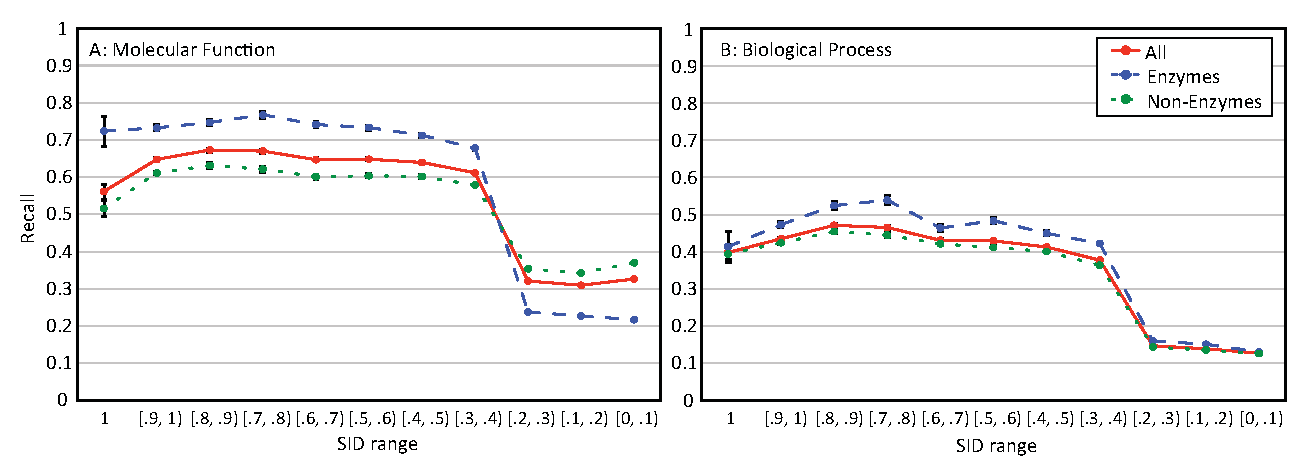
\includegraphics[width=\linewidth]{Figures/fanngo/Figure_3}
%\par\end{centering}
%\caption[Accuracy of function transfer using global pairwise sequence identities for enzymes vs. non-enzymes]{Accuracy of function transfer using global pairwise sequence identities for enzymes vs. non-enzymes (A: Molecular Function; B: Biological Process). For each sequence identity range (x-axis), shown is the average precision of function transfer by pairwise similarity (blue dashed line: enzymes, green dotted line: non-enzymes; red solid line: combined). The error bars represent 95\% confidence intervals}
%\label{fig:fanngo3}
%\end{figure*}
%%%%%%%%%%%%%%%%%%%%%%
%%%%%%%%%%%%%%%%%%%%%%
%
%Another interesting trend in the data is the fact that the quality of annotations transferred between sequences from the same species is higher than that obtained between different species. This can be seen by comparing the precision/recall curves in \Cref{fig:fanngo4} obtained by only considering pairs of sequences from the same species (``within" curve, blue line), and only considering pairs of sequences from different organisms (``between" curve, green line). A similar trend has been previously observed on protein-protein interaction data by \citep{Mika2006}.
%
%%%%%%%%%%%%%%%%%%%%%%
%%%%%%%%%%%%%%%%%%%%%%
%\begin{figure*}[h!]
%\begin{centering}
%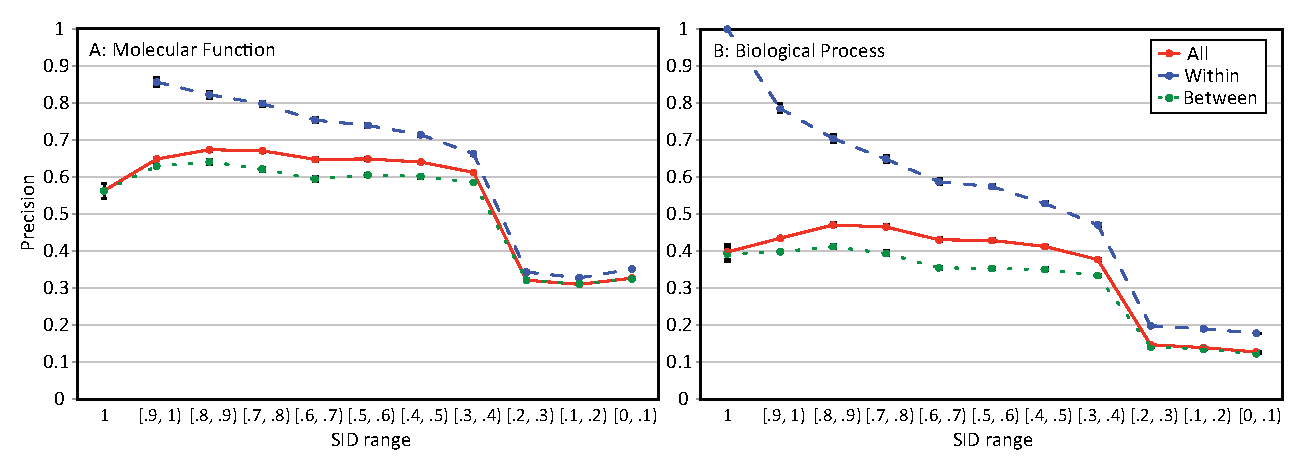
\includegraphics[width=\linewidth]{Figures/fanngo/Figure_4}
%\par\end{centering}
%\caption[Accuracy of function transfer using global pairwise sequence identities from the same or different organism]{Accuracy of function transfer using global pairwise sequence identities from the same or different organism (A: Molecular Function; B: Biological Process). For each sequence identity range (x-axis), shown is the average precision of function transfer by pairwise similarity (blue dashed line: same organism, green dotted line: different organism; red solid line: combined). The error bars represent 95\% confidence intervals.}
%\label{fig:fanngo4}
%\end{figure*}
%%%%%%%%%%%%%%%%%%%%%%
%%%%%%%%%%%%%%%%%%%%%%
%
%%%%%%%%%%%%%%%%%%%%%%
%%%%%%%%%%%%%%%%%%%%%%
%\subsection{Quality of non-experimental annotations in Swiss-Prot}
%%%%%%%%%%%%%%%%%%%%%%
%%%%%%%%%%%%%%%%%%%%%%
%
%Protein databases such as GO or Swiss-Prot contain a number of functional annotations supported by non-experimental evidence codes. We aimed to assess the quality of such annotations by analyzing non-experimental annotations for the proteins in Swiss-Prot (v10.0-v15.0) that in a later release (v15.15) accumulated experimental annotations.  \Cref{fig:fanngo5} shows the quality of annotations by non-traceable author statement (NAS) or inferred from electronic annotation (IEA) evidence codes (the remaining non-experimental codes did not contain enough sequences). Using the current annotations (v15.15) as true function, the precision and recall of each protein's annotation were calculated (\Cref{fig:fanngo5}). 
%
%%%%%%%%%%%%%%%%%%%%%%
%%%%%%%%%%%%%%%%%%%%%%
%\begin{figure*}[h!]
%\begin{centering}
%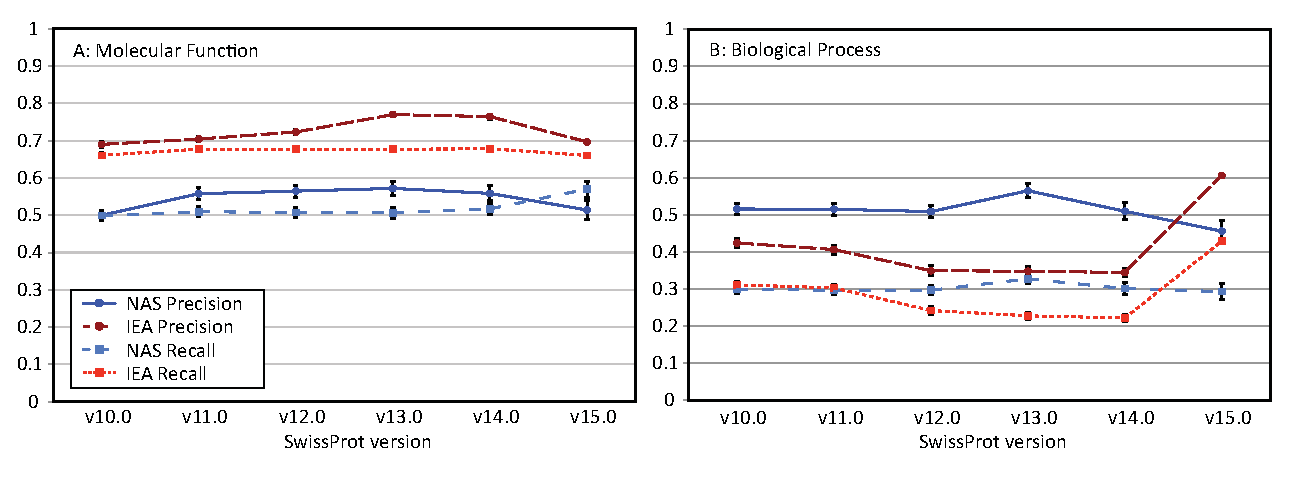
\includegraphics[width=\linewidth]{Figures/fanngo/Figure_5}
%\par\end{centering}
%\caption[Accuracy of function transfer between different versions of the Swiss-Prot database]{Accuracy of function transfer for the Swiss-Prot database (A: Molecular Function; B: Biological Process). X-axis represents a different version of Swiss-Prot. The dark dashed red line represents the precision of IEA annotations and the dark blue solid line represents the precision of NAS annotations. The light red dotted line represents the recall of IEA annotations, and the light blue dashed line represents the recall of NAS annotations. The error bars represent 95\% confidence intervals.}
%\label{fig:fanngo5}
%\end{figure*}
%%%%%%%%%%%%%%%%%%%%%%
%%%%%%%%%%%%%%%%%%%%%%
%
%As shown in \Cref{fig:fanngo5}, the quality of electronic annotations is consistently better than that of non-traceable author statements for MFO, while the trend is reversed for BPO. Interestingly, the precision of the electronic annotations in the Swiss-Prot database for MFO exceeds the level achieved  (\Cref{fig:fanngo2}), while the NAS evidence suggest lower confidence levels compared to that of sequence transfer. A historical analysis of BPO annotations suggests that neither electronic annotation, nor non-traceable author statements, have been at the level of simple transfer of annotation; however the latest major release of Swiss-Prot (v15.0) provides more accurate electronic inference than transfer by sequence similarity.
%